\documentclass[spec, och, otchet, hidelinks]{SCWorks}
% параметр - тип обучения - одно из значений:
%    spec     - специальность
%    bachelor - бакалавриат (по умолчанию)
%    master   - магистратура
% параметр - форма обучения - одно из значений:
%    och   - очное (по умолчанию)
%    zaoch - заочное
% параметр - тип работы - одно из значений:
%    otchet
%    referat    - реферат
%    coursework - курсовая работа (по умолчанию)
%    diploma    - дипломная работа
%    pract      - отчет по практике
%    pract      - отчет о научно-исследовательской работе
%    autoref    - автореферат выпускной работы
%    assignment - задание на выпускную квалификационную работу
%    review     - отзыв руководителя
%    critique   - рецензия на выпускную работу
% параметр - включение шрифта
%    times    - включение шрифта Times New Roman (если установлен)
%               по умолчанию выключен
\usepackage[T2A]{fontenc}
\usepackage[utf8]{inputenc}
\usepackage{graphicx}

\usepackage[sort,compress]{cite}
\usepackage{amsmath}
\usepackage{amssymb}
\usepackage{amsthm}
\usepackage{fancyvrb}
\usepackage{longtable}
\usepackage{array}
\usepackage[english,russian]{babel}
\usepackage{listings}
\usepackage{xcolor}
% Используется автором репозитория
%\usemintedstyle{xcode}
% Этот пакет включает в себя аналогичный Times New Roman шрифт.
% Необходим для успешной компиляции для UNIX-систем ввиду отсутствия TNR в нем.
% Можно использовать и для Windows.
\usepackage{tempora}

\lstset{%
	language=C,
	backgroundcolor=\color{gray!12},
	basicstyle=\ttfamily\small,
	keywordstyle=\color{blue},
	stringstyle=\color{blue},
	showstringspaces=false,
	captionpos=b,
	numbers=left,
	numberstyle=\footnotesize\color{gray},
	frame=TB,
	tabsize=2,
	morekeywords={procedure, then, begin, end}
}

\usepackage[colorlinks=false]{hyperref}

\graphicspath{{figures/}}

\newcommand{\eqdef}{\stackrel {\rm def}{=}}

\usepackage{stackengine}
\newcommand\xrowht[2][0]{\addstackgap[.5\dimexpr#2\relax]{\vphantom{#1}}}
\newcommand{\tbf}[1]{\textbf{#1}}
\newtheorem{lem}{Лемма}

% % При использовании biblatex вместо bibtex
%\usepackage[style=gost-numeric]{biblatex}
%\addbibresource{thesis.bib}

\begin{document}

% Кафедра (в родительном падеже)
\chair{математической кибернетики и компьютерных наук}

% Тема работы
\title{Преобразователи кодов}

% Курс
\course{3}

% Группа
\group{331}

% Факультет (в родительном падеже) (по умолчанию "факультета КНиИТ")
%\department{факультета КНиИТ}

% Специальность/направление код - наименование
%\napravlenie{02.03.02 "--- Фундаментальная информатика и информационные технологии}
%\napravlenie{02.03.01 "--- Математическое обеспечение и администрирование информационных систем}
%\napravlenie{09.03.01 "--- Информатика и вычислительная техника}
%\napravlenie{09.03.04 "--- Программная инженерия}
\napravlenie{10.05.01 "--- Компьютерная безопасность}

% Для студентки. Для работы студента следующая команда не нужна.
%\studenttitle{Студентки}

% Фамилия, имя, отчество в родительном падеже
\author{Бородина Артёма Горовича}

% Заведующий кафедрой
\chtitle{доцент, к.\,ф.-м.\,н.} % степень, звание
\chname{С.\,В.\,Миронов}

%Научный руководитель (для реферата преподаватель проверяющий работу)
\satitle{аспирант}%, к.\,ф.-м.\,н.} %должность, степень, звание
\saname{А.\,А.\,Мартышкин}

% Руководитель практики от организации (только для практики,
% для остальных типов работ не используется)
\patitle{к.\,ф.-м.\,н., доцент}
\paname{Д.\,Ю.\,Петров}

% Семестр (только для практики, для остальных
% типов работ не используется)
\term{2}

% Наименование практики (только для практики, для остальных
% типов работ не используется)
\practtype{учебная}

% Продолжительность практики (количество недель) (только для практики,
% для остальных типов работ не используется)
\duration{2}

% Даты начала и окончания практики (только для практики, для остальных
% типов работ не используется)
\practStart{01.07.2016}
\practFinish{14.07.2016}

% Год выполнения отчета
\date{2022}

\maketitle

% Включение нумерации рисунков, формул и таблиц по разделам
% (по умолчанию - нумерация сквозная)
% (допускается оба вида нумерации)
%\secNumbering


\tableofcontents

% Раздел "Обозначения и сокращения". Может отсутствовать в работе
% \abbreviations
% \begin{description}
%     \item ... "--- ...
%     \item ... "--- ...
% \end{description}

% Раздел "Определения". Может отсутствовать в работе
%\definitions

% Раздел "Определения, обозначения и сокращения". Может отсутствовать в работе.
% Если присутствует, то заменяет собой разделы "Обозначения и сокращения" и "Определения"
%\defabbr


% Раздел "Введение"

\section{Цель работы и порядок выполнения}

Цель работы — изучение основных понятий универсальной алгебры и операций над бинарными отношениями.
\\

\par \textbf{Порядок выполнения работы}
\begin{enumerate}
\item Рассмотреть понятие алгебраической операции и классификацию свойств операций.
  Разработать алгоритмы проверки свойств операций: ассоциативность,
  коммутативность, идемпотентность, обратимость, дистрибутивность.
  
\item Рассмотреть основные операции над бинарными отношениями. Разработать
  алгоритмы выполнения операции над бинарными отношениями.
  
\item Рассмотреть основные операции над матрицами. Разработать алгоритмы
выполнения операций над матрицами.
\end{enumerate}

\newpage

\section{Теоретические сведения по рассмотренным темам с их обоснованием}

\par \textbf{Определение.} \textbf{Алгебраической $n$-арной операцией} называется
отображение $f: A^n \rightarrow A$ на множестве A. При этом $n$ называется
порядком или арностью алгебраической операции $f$.

\par \textbf{Классификация свойств операций.} \\
Бинарная операция $\cdot$ на множестве $A$ называется:

\begin{enumerate}
\item \textbf{Ассоциативной}, если $\forall x, y, z \in A$ выполняется
  равенство $x\cdot (y \cdot z) = (x \cdot y) \cdot z$;
\item \textbf{Коммутативной}, если $\forall x, y \in A$ выполняется равенство $x
  \cdot y = y \cdot x$;
\item \textbf{Идемпотентной}, если $\forall x \in A$ выполняется равенство $x
  \cdot x = x$;
\item \textbf{Обратимой}, если $\forall x, y \in A$ уравнения $x \cdot a = y$ и $b
  \cdot x = y$ имеют решение, причём единственное;
\item \textbf{Дистрибутивной относительно операции +}, если $\forall x, y, z \in
  A$ выполняются равенства $ x \cdot (y + z) = (x \cdot y) + (x \cdot z)$ и 
  $(y + z) \cdot x = (y \cdot x) + (z \cdot x)$. \\
\end{enumerate}

\par \textbf{Действия над бинарными отношениями.} \\
Определим следующие действия над бинарными отношениями:

\begin{enumerate}
\item \tbf{Пересечением} $P \cap Q$ отношений $P \subset A \times B$ и $Q \subset
  A \times B$ называется отношение, которое
  содержит только общие для $P$ и $Q$ пары: $P \cap Q = \{(x,
  y): (x, y) \in P \; \text{и} \; (x, y) \in Q\}$;
\item \tbf{Объединением} $P \cup Q$ отношений $P \subset A \times B$ и $Q
  \subset A \times B$ называется отношение, которое
  включает все пары, содержащиеся или в подмножестве $P$ или в подмножестве
  $Q: P \cup Q = \{(x, y): (x, y) \in P \; \text{или} \; (x, y) \in Q\}$.
  Когда объединение $P \cup Q$ содержит все возможные пары из $A \times B$, а
  пересечение $P$ и $Q$ пусто, то говорят, что отношения $P$ и $Q$
  \tbf{образуют разбиение} $A \times B$, а их объединение есть \tbf{полное
    отношение};
\item \tbf{Дополнением} $\overline P \subset A \times B$ отношения $P \subset A
  \times B$ называется отношение, состоящее из тех
  пар $(x, y) \in A \times B$, которые не входят в $P: \{(x, y): (x, y) \in
  A \times B \; \text{и} \; (x, y) \notin P\}$. Отношения $P \; \text{и} \;
  \overline P$ образуют \tbf{разбиение} $A \times B \, $, т.е. $\,P \cup \overline
  P = A \times B \; \text{и} \; P \cap \overline P = \varnothing$.
\item \tbf{Обратным отношением} $P^{-1} \subset B \times A$ к отношению $P
  \subset A \times B$ называется
  отношение, которое содержит пару $(x, y)$ тогда и только тогда, когда $(y,
  x) \in P$, т.е. $P^{-1} = \{(x, y): (y, x) \in P\}$;
\item \tbf{Композицией (произведением)} $P \circ Q$ отношений $P \subset A
  \times B$ и $Q \subset B \times C$
  называется отношение, которое содержит пару $(x, y)$ тогда и только тогда,
  когда существует $z \in B$ такое, что $(x, z) \in P$ и $(z, y) \in Q$,
  т.е. $P \circ Q = \{(x, y): \; \text{найдётся} \; z \; \text{такое, что}
  \; (x, z) \in P \; \text{и} \; (z, y) \in Q\}$. К частным случаям
  композиции относится \tbf{квадрат отношения} $P: P^2 = \{(x, y):
  \text{найдётся} \; z \; \text{такое, что} \; (x, z) \in P \; \text{и} \; (z, y)
  \in P\}$. По индукции определяется $n$-ая \tbf{степень отношения} $P: P^n
  = P^{n - 1} \circ P $.\\
\end{enumerate}

\par \tbf{Проверка ассоциативности операции по тесту Лайта.} \\
В случае конечного $n$-элементного множества $S = \{s_1, s_2, \dots, s_n\}$
операция умножения на $S$ задаётся \textit{таблицей Кэли} размерности $n \times
n$, строки и столбцы которой помечены элементами множества $S$ и в которой на
пересечении $i$-ой строки и $j$-го столбца стоит произведение $s_i \cdot s_j$
элементов $s_i, s_j$.

\begin{figure}[h]
  \center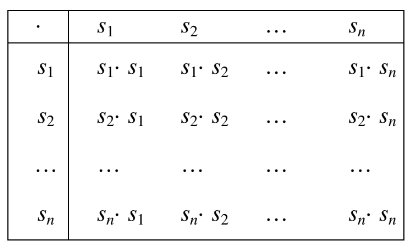
\includegraphics[scale=0.6]{cayley_table.png}
\end{figure}

\par Ассоциативность такой операции определяется по \textit{тесту Лайта}: для
доказательства тождества ассоциативности последовательно фиксируем элементы $a
\in S$ и проверяем выполнимость равенства: $(x \cdot a) \cdot z = x \cdot (a
\cdot z)$ для любых $x, z \in S$ путём сравнения следующих двух таблиц,
составленных для произведений соответственно левой и правой частей этого
равенства.

\newpage

\par Таблица произведений $(x \cdot a) \cdot z$ левой части равенства:

\begin{figure}[h]
  \center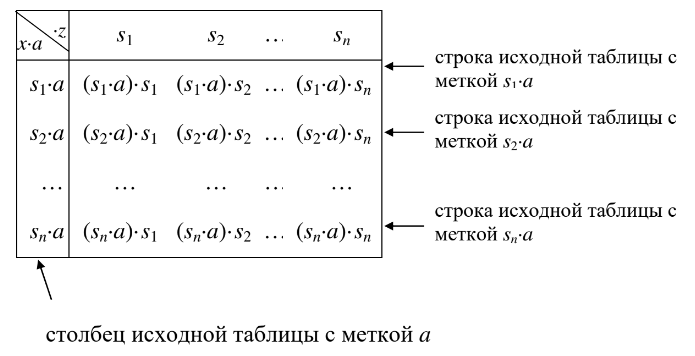
\includegraphics[scale=0.5]{left_cayley.png}
\end{figure}

\par Таблица произведений $x \cdot (a \cdot z)$ правой части равенства:

\begin{figure}[h]
  \center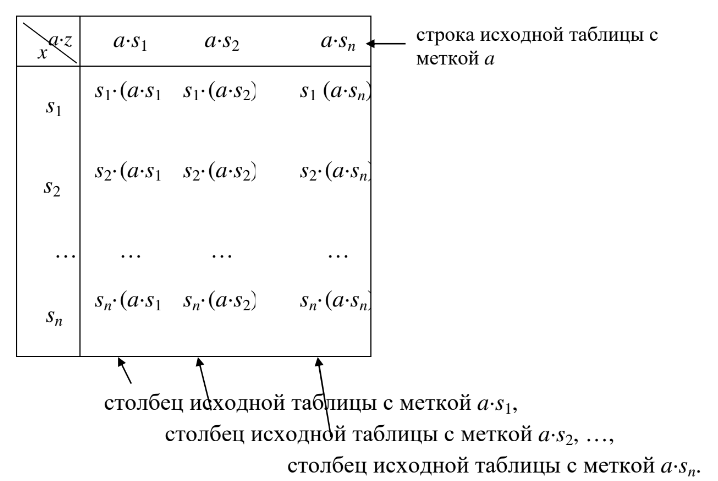
\includegraphics[scale=0.5]{right_cayley.png}
\end{figure}

\newpage

\section{Результаты работы}

\subsection{Алгоритм проверки свойства ассоциативности операции}
\par \tbf{Описание алгоритма проверки свойства ассоциативности операции.}
\tbf{Вход:} множество объектов $S$ и таблица Кэли рассматриваемой операции
$\cdot$ над множеством объектов. \\
\tbf{Выход:} сообщение 'Операция является ассоциативной.' или 'Операция не
является ассоциативной.' \\
\tbf{Метод:} Ассоциативность операции определяется по \textit{тесту Лайта}:
для доказательства тождества ассоциативности последовательно фиксируем элементы
$a \in S $ ($S$ -- конечное $n$-элементное множество объектов) и проверяем выполнимость равенства:
$(x \cdot a) \cdot z = x \cdot (a \cdot z)$ для любых $x, z \in S$ путем
сравнения таблиц произведений $(x \cdot a) \cdot z$ левой части равенства и $x
\cdot (a \cdot z)$ правой части равенства.

\par \tbf{Псевдокод алгоритма проверки свойства ассоциативности операции.}
\begin{lstlisting}[caption=Псевдокод алгоритма., mathescape]
check_associativity(<N\matrix N> CayleyTable, objectSet[])
{
  pair<<matrix>, <matrix>> tables;
  for object in objectSet:
  {
    tables = construct_tables(CayleyTable, object);
    if (tables.left != tables.right)
      return (false);
  }
  return (true);
}
\end{lstlisting}

\par \tbf{Код программы проверки свойства ассоциативности операции.}
\begin{lstlisting}[caption=Код программы., mathescape]
pair<vector<vector<int>>, vector<vector<int>>> constructTables (
  vector<vector<int>> CayleyTable, int object)
{
  int i, j;
  vector<vector<int>> leftTable (
    matrixDimension, vector<int>(matrixDimension, 0)), 
                      rightTable (
   matrixDimension, vector<int>(matrixDimension, 0));

  for (i = 0; i < matrixDimension; ++i)
    for (j = 0; j < matrixDimension; ++j)
      {
        leftTable[i][j] = 
          CayleyTable[CayleyTable[i][object - 1] - 1][j];
        rightTable[i][j] = 
          CayleyTable[i][CayleyTable[object - 1][j] - 1];
      }
  return (make_pair (leftTable, rightTable));
}

bool checkAssociativity (vector<vector<int>> CayleyTable)
{
  int i;
  pair<vector<vector<int>>, vector<vector<int>>> tables;

  for (i = 0; i < objectSet.size (); ++i)
    {
      tables = constructTables (CayleyTable, objectSet[i]);
      if (tables.first != tables.second)
        return (false);
    }
  return (true);
}
\end{lstlisting}

\par \tbf{Оценка временной сложности алгоритма проверки свойства ассоциативности
  операции.}
\par Алгоритм был реализован наивно -- он заключается в проверке всех возможных
троек аргументов путём построения и сравнения элементов левой и правой таблиц
произведений. Такая реализация требует $O(n^3)$ времени, где $n$ -- размер
множества объектов, над которым определена операция. 

\newpage

\subsection{Алгоритм проверки свойства коммутативности операции}
\par \tbf{Описание алгоритма проверки свойства коммутативности операции.} \\
\tbf{Вход:} множество объектов $S$ и таблица Кэли $CayleyTable$ рассматриваемой операции
$\cdot$ над множеством объектов. \\
\tbf{Выход:} сообщение 'Операция является коммутативной.' или 'Операция не
является коммутативной.' \\
\tbf{Метод:} проверяются только элементы, для которых $j \geq  i$ ($i = 1,\dots,N,
\; j = 1,\dots,N, \; N$ -- размер множества объектов) -- элементы, расположенные
над главной диагональю в таблице Кэли. Между собой проверяются значения
элементов $CayleyTable[i][j]$ и $CayleyTable[j][i]$. Если все пары рассмотренных
элементов равны между собой, то операция коммутативна, иначе некоммутативна.

\par \tbf{Псевдокод алгоритма проверки свойства коммутативности операции.}
\begin{lstlisting}[caption=Псевдокод алгоритма., mathescape]
check_commutativity (<N\timesN matrix> CayleyTable)
{
  for (i = 0; i < N; ++i)
    for (j = i; j < N; ++j)
      if (CayleyTable[i][j] != CayleyTable[j][i])
        return false;
  return true;
}
\end{lstlisting}

\par \tbf{Код программы проверки свойства коммутативности операции.}
\begin{lstlisting}[caption=Код программы., mathescape]
bool checkCommutativity (vector<vector<int>> CayleyTable)
{
  int i, j;

  for (i = 0; i < CayleyTable.size(); ++i)
    for (j = i; j < CayleyTable.size(); ++j)
      if (CayleyTable[i][j] != CayleyTable[j][i])
        return (false);
  return (true);
}
\end{lstlisting}

\newpage

\par \tbf{Оценка временной сложности алгоритма проверки свойства коммутативности
  операции.}
\par Рассмотрим таблицу Кэли $CayleyTable$ операции $\cdot$ над множеством
объектов $S$ размера $n$. В первой строке таблице Кэли осуществляется $n$
проверок, во второй $n - 1$ и т.д. вплоть до последней строки таблицы, где
осуществляется одна проверка. Но $1 + 2 + \dots + n = (n^2 + n) / 2$. Таким
образом, оценка временной сложности алгоритма проверки коммутативности операции
$\cdot$ принимает вид: $O((n^2 + n) / 2) = O(n^2)$.

\newpage

\subsection{Алгоритм проверки свойства идемпотентности операции}
\par \tbf{Описание алгоритма проверки свойства идемпотентности операции.} \\
\tbf{Вход:} множество объектов $S$ и таблица Кэли $CayleyTable$ рассматриваемой операции
$\cdot$ над множеством объектов. \\
\tbf{Выход:} множество идемпотентов операции $\cdot$ и сообщение 'Операция
является идемпотентой.' или 'Операция не
является идемпотентной.' \\
\tbf{Метод:} проверка на идемпотентность осуществляется проходом по главной
диагонали таблицы Кэли. Элемент $x \in S$ называется идемпотентом операции $\cdot$,
если $x \cdot x = x$. Операция называется идемпотентной, если все объекты, над
которой она определена -- идемпотенты этой операции. В случае идемпотентности
элемента $x \in S$ он заносится в множество идемпотентов этой операции, которое
затем выводится.

\par \tbf{Псевдокод алгоритма проверки свойства идемпотентности операции.}
\begin{lstlisting}[caption=Псевдокод алгоритма., mathescape]
check_idempotency(<N\times N matrix> CayleyTable, objectSet[])
{
  idempotents[];
  for i in range(N):
    if (CayleyTable[i][i] == objectSet[i])
      idempotents.push_back(objectSet[i]);
  print(idempotents);
  return (N == idempotents.size());
}
\end{lstlisting}

\par \tbf{Код программы проверки свойства идемпотентности операции.}
\begin{lstlisting}[caption=Код программы., mathescape]
bool checkIdempotency (vector<vector<int>> CayleyTable)
{
  int i;
  vector<int> idempotents;

  for (i = 0; i < matrixDimension; ++i)
    if (CayleyTable[i][i] == objectSet[i])
      idempotents.push_back (objectSet[i]);

  int idSize = idempotents.size ();
  cout << "IDEMPOTENTS OF THIS OPERATION ";
  if (idSize == 0)
    cout << "IS: EMPTY SET.\n";
  else if (idSize == 1)
    cout << "IS: " << idempotents[0] << ".\n";
  else if (idSize == objectSet.size ())
    cout << "IS: OBJECT SET. ";
  else
    {
      cout << "ARE: ";
      for (i = 0; i < idSize; ++i)
        cout << idempotents[i] << 
          (i == idSize - 1 ? ". " : ", ");
    }
  return (idSize == objectSet.size ());
}
\end{lstlisting}

\par \tbf{Оценка временной сложности алгоритма проверки свойства идемпотентности
  операции.}
\par Рассмотрим таблицу Кэли размерности $N\times N$ операции $\cdot$. Временная
сложность алгоритма проверки свойства идемпотентности операции: $O(N)$, т.к.
проход осуществляется только по элементам главной диагонали таблицы Кэли.

\par \tbf{Результат тестирования программы проверки свойств заданной операции.}
\par Рассмотрим операцию $\cdot$ со своей таблицей Кэли размерности $N\times N$.
Проверим свойства ассоциативности, коммутативности и идемпотентности заданной
операции $\cdot$.

\begin{figure}[h]
  \center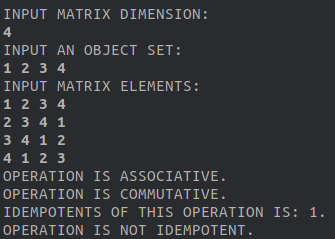
\includegraphics[scale=0.65]{check_properties.png}
  \caption{Результат проверки свойств заданной операции $\cdot$.}
\end{figure}

\par Как видно, рассматриваемая нами операция $\cdot$ является коммутативной и
ассоциативной, но не является идемпотентной.

\newpage

\subsection{Алгоритм проверки свойства дистрибутивности операции}
\par \tbf{Описание алгоритма проверки свойства дистрибутивности операции.} \\
\tbf{Вход:} множество объектов $S$ и таблицы Кэли операций $+$ и $\cdot$ над
этим множеством объектов. \\
\tbf{Выход:} сообщение о том, является ли операция $\cdot$ право-, лево- или
просто дистрибутивной относительно операции $+$. \\
\tbf{Метод:} сначала операция $\cdot$ проверяется на коммутативность. Если
операция коммутативна и дистрибутивна, то она и леводистрибутивна, и
праводистрибутивна. Если же операция не будет коммутативна, то она может
оказаться как только леводистрибутивной, так и только праводистрибутивной. Для
каждого элемента $x$ из множества объектов $S$ строятся таблицы вида $(b + c)
\cdot x$ и $(b \cdot x) + (c \cdot x)$ -- для проверки правой дистрибутивности и
$x \cdot (b + c)$ и $(x \cdot b) + (x \cdot c)$ -- для проверки левой
дистрибутивности. Если операция коммутативна, то неважно, какую из таблиц строить. \\

\par \tbf{Псевдокод алгоритма проверки свойства дистрибутивности операции.}
\begin{lstlisting}[caption=Псевдокод алгоритма., mathescape]
check_distributivity(<N$\times$N matrix> multCayTab, 
  <N$\times$N matrix> addCayTab, objectSet[])
{
  bool leftDistributive = rightDistributive = true;

  if (check_commutativity(multCayTab))
  {
    for object in objectSet:
      if construct_left_tables(
           multCayTab, addCayTab, object) are not equal:
        print('Distributive.');
    print('Not distributive.');
  }
  else 
  {
    for object in objectSet:
      if construct_left_tables(
           multCayTab, addCayTab, object) are not equal
      {
        leftDistributive = false;
        print('Not left-distributive.');
        break;
      }
    if (leftDistributive)
      print('Left-distributive.');
      
    for object in objectSet:
      if construct_right_tables(
           multCayTab, addCayTab, object) are not equal
      {
        rightDistributive = false;
        print('Not right-distributive.');
        break;
      }
    if (rightDistributive)
      print('Right-distributive');
    if (leftDistributive and rightDistributive)
      print('Distributive.');
  }
}
\end{lstlisting}

\par \tbf{Код программы проверки свойства дистрибутивности операции.}
\begin{lstlisting}[caption=Код программы., mathescape]
bool constructLeftTables (vector<vector<int>> mCT, 
                          vector<vector<int>> aCT, int curEl)
{
  int j, k;
  vector<vector<int>> 
    lTable (matrixDimension, vector<int> (matrixDimension, 0)),
    rTable (matrixDimension, vector<int> (matrixDimension, 0));
  for (j = 0; j < matrixDimension; ++j)
    for (k = 0; k < matrixDimension; ++k)
      {
        lTable[j][k] = mCT[curEl][aCT[j][k]];
        rTable[j][k] = aCT[mCT[curEl][j]][mCT[curEl][k]];
      }
  return (lTable == rTable);
}

bool constructRightTables (vector<vector<int>> mCT, 
                           vector<vector<int>> aCT, int curEl)
{
  int j, k;
  vector<vector<int>> 
    lTable (matrixDimension, vector<int> (matrixDimension, 0)),
    rTable (matrixDimension, vector<int> (matrixDimension, 0));
  for (j = 0; j < matrixDimension; ++j)
    for (k = 0; k < matrixDimension; ++k)
      {
        lTable[j][k] = mCT[aCT[j][k]][curEl];
        rTable[j][k] = aCT[mCT[j][curEl]][mCT[k][curEl]];
      }
  return (lTable == rTable);
}

void checkDistributivityMachinerie (
  vector<vector<int>> mCT, vector<vector<int>> aCT)
{
  int i, j, k;
  bool flagL = true, flagR = true;
  if (checkCommutativity (mCT))
    {
      for (i = 0; i < matrixDimension; ++i)
        if (!constructLeftTables (mCT, aCT, i))
          {
            cout << "OPERATION IS NOT DISTRIBUTIVE.\n";
            return;
          }
      cout << "OPERATION IS DISTRIBUTIVE.\n";
    }
  else
    {
      for (i = 0; i < matrixDimension; ++i)
        if (!constructLeftTables (mCT, aCT, i))
          {
            cout << "OPERATION IS NOT LEFT-DISTRIBUTIVE.\n";
            flagL = false;
            break;
          }
      if (flagL)
        cout << "OPERATION IS LEFT-DISTRIBUTIVE.\n";

      for (i = 0; i < matrixDimension; ++i)
        if (!constructRightTables (mCT, aCT, i))
          {
            cout << "OPERATION IS NOT RIGHT-DISTRIBUTIVE.\n";
            flagR = false;
            break;
          }
      if (flagR)
        cout << "OPERATION IS RIGHT-DISTRIBUTIVE.\n";
      if (flagL && flagR)
        cout << "OPERATION IS DISTRIBUTIVE.\n";
    }
}
\end{lstlisting}

\par \tbf{Результат тестирования программы проверки свойства дистрибутивности
  операции.}
\par Рассмотрим таблицы Кэли операций $+$ и $\cdot$. Проверим дистрибутивность
операции $\cdot$ относительно операции $+$.

\begin{figure}[h]
  \center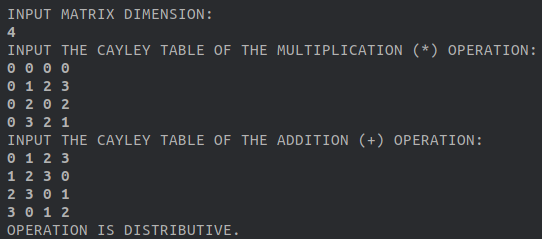
\includegraphics[scale=0.6]{check_distr.png}
  \caption{Результат проверки свойства дистрибутивности операции $\cdot$
    относительно операции $+$.}
\end{figure}

\par Как видно, операция $\cdot$ является дистрибутивной относительно операции $+$.

\par \tbf{Оценка сложности алгоритма проверки свойства дистрибутивности
  операции.}
\par Аналогично алгоритму проверки ассоциативности, в этом алгоритме происходит
сравнение всех троек аргументов и сравнение элементов правых и левых таблиц
дистрибутивности. Временная сложность алгоритма: $O(n^3)$, где $n$ -- размер
множества объектов, над которым определены операции $\cdot$ и $+$.

\newpage

\subsection{Алгоритм объединения бинарных отношений}
\par \tbf{Описание алгоритма объединения бинарных отношений.} \\
\tbf{Вход:} матрицы $A$ и $B$ (одинаковой размерности $N \times M$) бинарных отношений $\rho$ и $\delta$. \\
\tbf{Выход:} матрица $A \cup B$ размерности $N \times M$ бинарного отношения
$\rho \cup \delta$. \\
\tbf{Метод:} вычисляется результат применения операции <<логическое ИЛИ>> к
элементам матриц $A$ и $B$, расположенным на пересечении $i$-ой строки и $j$-го
столбца ($i = 1,\dots,N, \; j = 1,\dots,M$). Результат применения операции
заносится в соответствующую ячейку матрицы $A \cup B$. \\

\par \tbf{Псевдокод алгоритма объединения бинарных отношений.}

\begin{lstlisting}[caption=Псевдокод алгоритма., mathescape]
binary_relation_union(<N$\times$M matrix> fBinRelMat,
                      <N$\times$M matrix> sBinRelMat)
{
  <N$\times$M matrix> binRelUnion;
  for i in range(N):
    for j in range(M):
      if (fBinRelMat[i][j] == 1) || (sBinRelMat[i][j] == 1):
        then binRelUnion[i][j] = 1; else binRelUnion[i][j] = 0;
  return (binRelUnion);
}
\end{lstlisting}

\par \tbf{Код программы объединения бинарных отношений.}
\begin{lstlisting}[caption=Код программы., mathescape]
vector<vector<int>> getBinaryRelationUnion (
  vector<vector<int>> fM, vector<vector<int>> sM)
{
    int i, j, rowsNum = fM.size (), colsNum = fM[0].size ();
    vector<vector<int>> unionMatrix (
      rowsNum, vector<int> (colsNum, 0));

    for (i = 0; i < rowsNum; ++i)
        for (j = 0; j < colsNum; ++j)
            unionMatrix[i][j] = ((fM[i][j] == 1) || 
                                 (sM[i][j] == 1) ? 1 : 0);
    return (unionMatrix);
}
\end{lstlisting}

\par \tbf{Результат тестирования программы объединения бинарных отношений.}
\par Рассмотрим пару бинарных отношений $\rho$ и $\delta$, заданных матрицами
размерности 4 $\times$ 3. Применим операцию объединения к бинарным отношениям
$\rho$ и $\delta$.
\begin{figure}[h]
  \center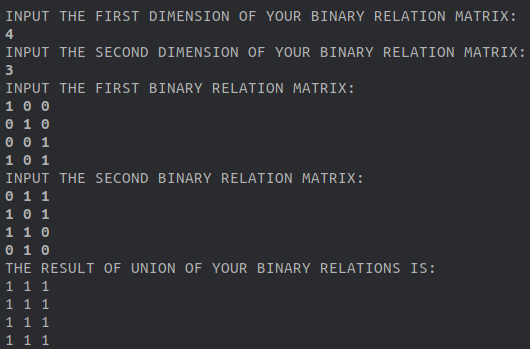
\includegraphics[scale=0.7]{binary_relation_union.png}
  \caption{Результат построения объединения бинарных отношений $\rho$ и $\delta$.}
\end{figure}

В результате работы программы была сформирована матрица бинарного отношения
$\rho \cup \delta$. \\

\par \tbf{Оценка сложности алгоритма объединения бинарных отношений.}

\par Для формирования матрицы $A \cup B$ бинарного отношения $\rho \cup \delta$
требуется произвести операции над каждым элементом матриц $A$ и $B$. Общее число
элементов в каждой матрице -- $N \times M$, откуда и следует оценка временной
сложности алгоритма: $T(get\_binary\_relation\_union) = O(N \cdot M)$.

\newpage

\subsection{Алгоритм пересечения бинарных отношений}
\par \tbf{Описание алгоритма пересечения бинарных отношений.} \\
\tbf{Вход:} матрицы $A$ и $B$ (одинаковой размерности $N \times M$) бинарных отношений $\rho$ и $\delta$. \\
\tbf{Выход:} матрица $A \cap B$ размерности $N \times M$ бинарного отношения
$\rho \cap \delta$. \\
\tbf{Метод:} вычисляется результат применения операции <<логическое И>> к
элементам матриц $A$ и $B$, расположенным на пересечении $i$-ой строки и $j$-го
столбца ($i = 1,\dots,N, \; j = 1,\dots,M$). Результат применения операции
заносится в соответствующую ячейку матрицы $A \cap B$. \\

\par \tbf{Псевдокод алгоритма объединения бинарных отношений.}

\begin{lstlisting}[caption=Псевдокод алгоритма., mathescape]
binary_relation_intersection(<N$\times$M matrix> fBinRelMat,
                             <N$\times$M matrix> sBinRelMat)
{
  <N$\times$M matrix> binRelIntersection;
  for i in range(N):
    for j in range(M):
      if (fBinRelMat[i][j] == 1) && (sBinRelMat[i][j] == 1):
        then binRelIntersection[i][j] = 1; 
        else binRelIntersection[i][j] = 0;
  return (binRelIntersection);
}
\end{lstlisting}

\par \tbf{Код программы объединения бинарных отношений.}
\begin{lstlisting}[caption=Код программы., mathescape]
vector<vector<int>> getBinaryRelationIntersection (
  vector<vector<int>> fM, vector<vector<int>> sM)
{
  int i, j, rowsNum = fM.size (), colsNum = fM[0].size ();
  vector<vector<int>> intersectionMatrix (
    rowsNum, vector<int> (colsNum, 0));
  for (i = 0; i < rowsNum; ++i)
    for (j = 0; j < colsNum; ++j)
      intersectionMatrix[i][j] = ((fM[i][j] == 1) && 
                                  (sM[i][j] == 1) ? 1 : 0);
  return (intersectionMatrix);
}
\end{lstlisting}

\par \tbf{Результат тестирования программы пересечения бинарных отношений.}
\par Рассмотрим пару бинарных отношений $\rho$ и $\delta$, заданных матрицами
размерности 3 $\times$ 4. Применим операцию пересечения к бинарным отношениям
$\rho$ и $\delta$.
\begin{figure}[h]
  \center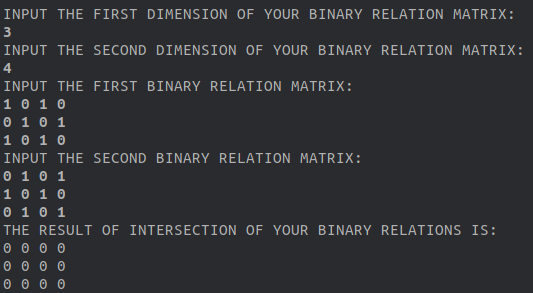
\includegraphics[scale=0.7]{binary_relation_intersection.png}
  \caption{Результат построения пересечения бинарных отношений $\rho$ и $\delta$.}
\end{figure}

В результате работы программы была сформирована матрица бинарного отношения
$\rho \cap \delta$. \\

\par \tbf{Оценка сложности алгоритма пересечения бинарных отношений.}

\par Для формирования матрицы $A \cap B$ бинарного отношения $\rho \cap \delta$
требуется произвести операции над каждым элементом матриц $A$ и $B$. Общее число
элементов в каждой матрице -- $N \times M$, откуда и следует оценка временной
сложности алгоритма: $T(get\_binary\_relation\_intersection) = O(N \cdot M)$.

\newpage

\subsection{Алгоритм построения дополнения бинарного отношения}
\par \tbf{Описание алгоритма построения дополнения бинарного отношения.} \\
\tbf{Вход:} матрица $A$ размерности $N \times M$ бинарного отношения $\rho$. \\
\tbf{Выход:} матрица $\overline A$ размерности $N \times M$ бинарного отношения
$\overline \rho$. \\
\tbf{Выход:} к каждому элементу матрицы $A$, стоящему на пересечении $i$-й
строки и $j$-го столбца ($i = 1,\dots,N, \; j = 1,\dots,M$), применяется
операция <<логическое НЕ>> (единица заменяется на ноль и наоборот). Результат
применения операции заносится в соответствующую ячейку матрицы $\overline A$. \\

\par \tbf{Псевдокод алгоритма построения дополнения бинарного отношения.}

\begin{lstlisting}[caption=Псевдокод алгоритма., mathescape]
binary_relation_complement(<N$\times$M matrix> BinRelMat)
{
  <N$\times$M matrix> binRelComplement;
  for i in range(N):
    for j in range(M):
      binRelComplement[i][j] = $\neg$binRelMat[i][j]
  return (binRelIntersection);
}
\end{lstlisting}

\par \tbf{Код программы построения дополнения бинарного отношения.}
\begin{lstlisting}[caption=Код программы., mathescape]
vector<vector<int>> getBinaryRelationComplement (
  vector<vector<int>> binRelMat)
{
  int i, j, rowsNum = binRelMat.size (), 
            colsNum = binRelMat[0].size ();
  vector<vector<int>> complementMatrix (
    rowsNum, vector<int> (colsNum, 0));

  for (i = 0; i < rowsNum; ++i)
    for (j = 0; j < colsNum; ++j)
      complementMatrix[i][j] = 1 - binRelMat[i][j];
  return (complementMatrix);
}
\end{lstlisting}

\newpage

\par \tbf{Результат тестирования программы построения дополнения бинарного
  отношения.}
\par Рассмотрим бинарное отношение $\rho$, заданное матрицей $A$ размерности 3
$\times$ 4. Построим дополнение $\overline \rho$ заданного бинарного отношения
$\rho$.

\begin{figure}[h]
  \center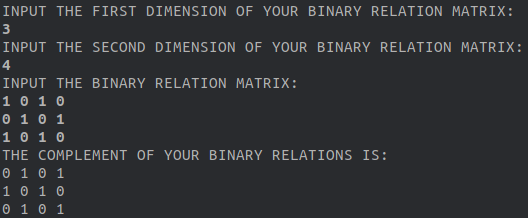
\includegraphics[scale=0.7]{binary_relation_complement.png}
  \caption{Результат построения дополнения бинарного отношения $\rho$.}
\end{figure}

\par В результате работы программы было построено бинарное отношение $\overline
\rho$ с получившейся матрицей $\overline A$ размерности 3 $\times$ 4. \\

\par \tbf{Оценка временной сложности алгоритма построения дополнения бинарного
  отношения.}
\par Поскольку в ходе работы программы обрабатывается каждый элемент некоторой
матрицы $A$ размерности $N \times M$, то из этого получаем временную оценку
сложности алгоритма: $T(get\_binary\_relation\_complement) = O(N \cdot M)$.

\newpage

\subsection{Алгоритм построения композиции бинарных отношений}
\par \tbf{Описание алгоритма построения композиции бинарных отношений.} \\
\tbf{Вход:} матрица $A$ размерности $N \times M$ и матрица $B$ размерности $L
\times K$ бинарных отношений $\rho$ и $\delta$. \\
\tbf{Выход:} сообщение об ошибке, в случае если $M$ не равно $L$, или матрица $A
\circ B$ размерности $N \times K$ бинарного отношения $\rho \circ \delta$. \\
\tbf{Метод:} будем считать, что $M$ и $L$ совпали. Тогда строим матрицу $A \circ
B$ путём обычного перемножения матриц $A$ и $B$: $A \cdot B$, а затем проверяем
каждый элемент получившейся матрицы, стоящий на пересечении $i$-ой строки и
$j$-го столбца ($i = 1,\dots,N, \; j = 1,\dots,K$) на то, больше ли он единицы.
Если да, то заменяем этот элемент на единицу, если нет, то оставляем без
изменения. 

\par \tbf{Псевдокод алгоритма построения композиции бинарных отношений.}
\begin{lstlisting}[caption=Псевдокод алгоритма., mathescape]
binary_relation_composition(<N$\times$M matrix> fBinRelMat,
                            <L$\times$K matrix> sBinRelMat)
{
  if M != L:
    return <<Wrong Input>>;

  <N $\times$ K matrix> boolMultiplicationMatrix, int product;
  for i in range(N):
    for j in range(K):
    {
      product = 0;
      for k in range(M):
        product += fBinRelMat[i][k] * sBinRelMat[k][j];
      if (product > 0):
      then boolMultiplicationMatrix[i][j] = 1;
      else boolMultiplicationMatrix[i][j] = 0;
    }
  return (boolMultiplicationMatrix);
}
\end{lstlisting}

\par \tbf{Код программы построения композиции бинарных отношений.}
\begin{lstlisting}[caption=Код программы., mathescape]
vector<vector<int>> getBinaryRelationMultiplication (
  vector<vector<int>> fBinRel, vector<vector<int>> sBinRel)
{
  int i, j, k, product, rowsNum = fBinRel.size (), 
                        colsNum = sBinRel[0].size ();
  vector<vector<int>> boolMultiplicationMatrix (
    rowsNum, vector<int> (colsNum, 0));

  for (i = 0; i < rowsNum; ++i)
    for (j = 0; j < colsNum; ++j)
      {
        product = 0;
        for (k = 0; k < fBinRel[0].size (); ++k)
          product += fBinRel[i][k] * sBinRel[k][j];
        boolMultiplicationMatrix[i][j] = (product > 0 ? 1 : 0);
      }
  return (boolMultiplicationMatrix);
}
\end{lstlisting}

\par \tbf{Результат тестирования программы построения композиции бинарных
  отношений.}
\par Рассмотрим бинарные отношения $\rho$ и $\delta$, заданные матрицами $A$ и
$B$ размерности 3 $\times$ 4 и 4 $\times$ 5. Построим композицию этих бинарных
отношений.

\begin{figure}[h]
  \center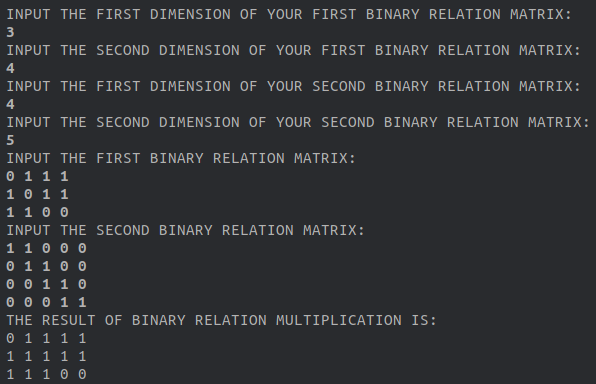
\includegraphics[scale=0.7]{binary_relation_composition.png}
  \caption{Результат построения композиции бинарных отношений.}
\end{figure}

\par В ходе выполнения программы была построена матрица $A \circ B$ размерности
3 $\times$ 5, соответствующая бинарному отношению $\rho \circ \delta$.

\par \tbf{Оценка временной сложности алгоритма построения композиции бинарных
  отношений.} 
\par Рассмотрим матрицы $A$ размерности $N \times M$ и $B$ размерности $M \times
K$ бинарных отношений $\rho$ и $\delta$. В матрице $A \circ B$ композиции
бинарных отношений будет содержаться $N \times K$ элементов. Для вычисления
значения каждого элемента матрицы $A \circ B$, находящегося на пересечении
$i$-ой строки и $j$-го столбца ($i = 1,\dots,N, \; j = 1,\dots,K$), необходимо
поэлементно перемножить $i$-ую строку первой матрицы с $j$-ым столбцом второй
матрицы. Для нахождения значения такого произведения требуется осуществить $M$
операций. Из этого следует временная оценка сложности:
$T(get\_binary\_relation\_multiplication) = O(N \cdot M \cdot K)$.

\newpage

\subsection{Алгоритм обращения бинарного отношения}
\par \tbf{Описание алгоритма обращения бинарного отношения.} \\
\tbf{Вход:} матрица $A$ размерности $N \times M$ бинарного отношения $\rho$. \\
\tbf{Выход:} матрица $A^{T}$ размерности $M \times N$ бинарного отношения
$\rho^{-1}$. \\
\tbf{Метод:} необходимо осуществить транспонирование исходной матрицы $A$
бинарного отношения $\rho$.

\par \tbf{Псевдокод алгоритма обращения бинарного отношения.}
\begin{lstlisting}[caption=Псевдокод алгоритма., mathescape]
binary_relation_inversion(<N$\times$M matrix> binRelMat)
{
  return (transpose(binRelMat));
}
\end{lstlisting}

\par \tbf{Код программы обращения бинарного отношения.}
\begin{lstlisting}[caption=Псевдокод алгоритма., mathescape]
vector<vector<int>> transposeBinaryRelationMatrix (
  vector<vector<int>> binRelMat)
{
  int i, j;
  vector<vector<int>> transposedMatrix;

  for (i = 0; i < binRelMat[0].size (); ++i)
    {
      vector<int> column;
      for (j = 0; j < binRelMat.size (); ++j)
        column.push_back (binRelMat[j][i]);
      transposedMatrix.push_back (column);
    }
  return (transposedMatrix);
}
\end{lstlisting}

\newpage

\par \tbf{Результат тестирования программы обращения бинарного отношения.}
\par Рассмотрим бинарное отношение $\rho$, заданное матрицей $A$ размерности 3
$\times$ 4. Найдём обратное к этому отношение.

\begin{figure}[h]
  \center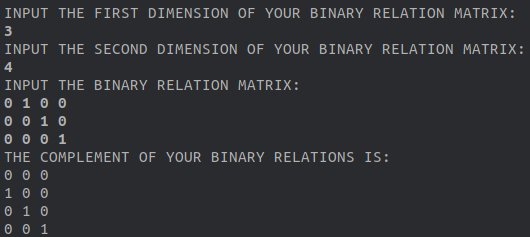
\includegraphics[scale=0.7]{binary_relation_inversion.png}
  \caption{Результат обращения бинарного отношения.}
\end{figure}

\par В результате работы программы была построена матрица $A^{T}$ размерности 4
$\times$ 3 бинарного отношения $\rho^{-1}$. \\

\par \tbf{Оценка временной сложности алгоритма обращения бинарного отношения.}
\par Оценим временную сложность алгоритма на примере матрицы $A$ размерности $N
\times M$ бинарного отношения $\rho$. После обращения бинарного отношения $\rho$
и построения бинарного отношения $\rho^{-1}$ число элементов в матрице $A^T$
будет соответствовать числу элементов в матрице $A$. Поскольку меняется только
размерность матрицы, а сами элементы лишь меняют своё расположение, то получаем
оценку временной сложности алгоритма: $T(get\_binary\_relation\_inversion) = O(N
\cdot M)$.

\newpage

\subsection{Алгоритм сложения матриц в конечном поле}
\par \tbf{Описание алгоритма сложения двух матриц в конечном поле.} \\
\tbf{Вход:} матрицы $A$ и $B$ размерности $N \times M$ над множеством
натуральных чисел и натуральное число $ord$ -- порядок поля. \\
\tbf{Выход:} матрица $A + B$ размерности $N \times M$ в конечном поле порядка
$ord$. \\
\tbf{Метод:} сложение матриц $A$ и $B$ осуществляется по обычному закону
сложения матриц. Затем в каждую ячейку, стоящую на пересечении $i$-ой строки и
$j$-го столбца ($i = 1,\dots,N, \; j = 1,\dots,M$) получившейся матрицы, записывается число
-- результат взятия остатка от деления рассматриваемого элемента на порядок поля.

\par \tbf{Псевдокод алгоритма сложения матриц в конечном поле.}
\begin{lstlisting}[caption=Псевдокод алгоритма., mathescape]
matrix_field_addition(<N$\times$M matrix> fMat,
                      <N$\times$M matrix> sMat,
                      unsigned int fieldOrder)
{
  <N$\times$M matrix> resMat;
  for i in range(N):
    for j in range(M):
      resMat[i][j] = (fMat[i][j] + sMat[i][j]) % fieldOrder;
  return (resMat);
}
\end{lstlisting}

\par \tbf{Код программы сложения матриц в конечном поле.}
\begin{lstlisting}[caption=Код программы., mathescape]
vector<vector<int>> addMatricesMachinerie (
  vector<vector<int>> lM,
  vector<vector<int>> rM, int fieldOrder)
{
  int i, j;
  vector<vector<int>> resM (
    lM.size (), vector<int> (lM[0].size (), 0));

  for (i = 0; i < lM.size (); ++i)
    for (j = 0; j < lM[i].size (); ++j)
      resM[i][j] = (lM[i][j] + rM[i][j]) % fieldOrder;
  return (resM);
}
\end{lstlisting}

\par \tbf{Результат тестирования программы сложения матриц в конечном поле.}

\par Рассмотрим матрицы $A$ и $B$ размерности 3 $\times$ 4 и порядок поля $ord$,
равный 8.

\begin{figure}[h]
  \center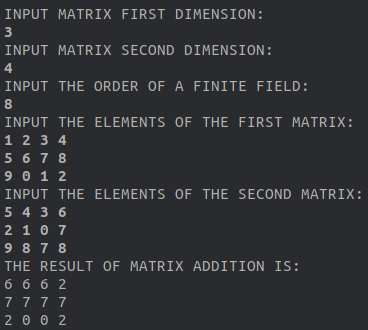
\includegraphics[scale=0.7]{matrix_field_addition.png}
  \caption{Результат сложения матриц в конечном поле порядка 8}.
\end{figure}

\par Результатом работы программы является матрица $A + B$ в конечном поле
порядка 8. \\

\par \tbf{Оценка временной сложности алгоритма сложения двух матриц в конечном
  поле.}

\par Для формирования матрицы $A + B$ в конечном поле порядка $ord$ требуется
произвести операции над каждым элементом матриц $A$ и $B$. Общее число
элементов в каждой матрице -- $N \times M$, откуда и следует оценка временной
сложности алгоритма: $T(get\_matrix\_field\_addition) = O(N \cdot M)$.

\newpage

\subsection{Алгоритм умножения матриц в конечном поле}
\par \tbf{Описание алгоритма умножения матриц в конечном поле.} \\
\tbf{Вход:} матрицы $A$ размерности $N \times M$ и $B$ размерности $L \times K$
над множеством натуральных чисел и натуральное число -- порядок поля $ord$. \\
\tbf{Выход:} сообщение об ошибке в случае, если размерность $M$ не совпадает с
$L$ или матрица $A \cdot B$ над конечным полем порядка $ord$. \\
\tbf{Метод:} в случае совпадения размерностей $M$ и $L$ умножение матриц $A$ и
$B$ осуществляется по обычному закону умножения матриц. Затем в каждую ячейку,
стоящую на пересечении $i$-ой строки и
$j$-го столбца ($i = 1,\dots,N, \; j = 1,\dots,K$) получившейся матрицы, записывается число
-- результат взятия остатка от деления рассматриваемого элемента на порядок поля.

\par \tbf{Псевдокод алгоритма умножения матриц в конечном поле.}
\begin{lstlisting}[caption=Псевдокод алгоритма., mathescape]
matrix_field_multiplication(<N$\times$M matrix> fMat,
                            <L$\times$K matrix> sMat)
{
  if M != L:
    return <<Wrong Input>>;

  <N $\times$ K matrix> multiplicationMat, int fieldOrder;
  for i in range(N):
    for j in range(K):
    {
      product = 0;
      for k in range(M):
        product += fMat[i][k] * sMat[k][j];
      multiplicationMat[i][j] = (product % fieldOrder);
    }
  return (multiplicationMat);
}
\end{lstlisting}

\par \tbf{Код программы умножения матриц в конечном поле.}
\begin{lstlisting}[caption=Код программы., mathescape]
vector<vector<int>> multiplyMatricesMachinerie (
  vector<vector<int>> lM, vector<vector<int>> rM, int fieldOrder)
{
  int i, j, k;
  vector<vector<int>> resM (lM.size (), 
                            vector<int> (rM[0].size (), 0));

  for (i = 0; i < lM.size (); ++i)
    for (j = 0; j < rM[0].size (); ++j)
      {
        int product = 0;
        for (k = 0; k < lM[0].size (); ++k)
          product += (lM[i][k] * rM[k][j]);
        resM[i][j] = (product % fieldOrder);
      }
  return (resM);
}
\end{lstlisting}

\par \tbf{Результат тестирования программы умножения матриц в конечном поле.}

\par Рассмотрим матрицы $A$ размерности 3 $\times$ 4 и $B$ размерности 4
$\times$ 3 и порядок поля $ord$, равный 13.

\begin{figure}[h]
  \center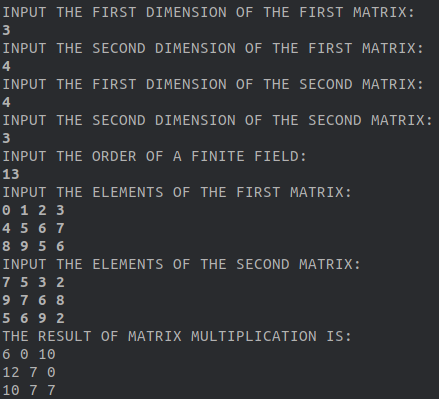
\includegraphics[scale=0.6]{matrix_field_multiplication.png}
  \caption{Результат умножения двух матриц в конечном поле порядка 13.}
\end{figure}

\par Результатом работы программы является матрица $A \cdot B$ размерности 3
$\times$ 3 в конечном поле порядка 13.

\newpage

\par \tbf{Оценка временной сложности алгоритма умножения матриц в конечном
  поле.}
\par Рассмотрим матрицы $A$ размерности $N \times M$ и $B$ размерности $M \times
K$ и порядок поля $ord$. В матрице $A \cdot B$ в конечном поле порядка $ord$
будет содержаться $N \times K$ элементов. Для вычисления
значения каждого элемента матрицы $A \cdot B$, находящегося на пересечении
$i$-ой строки и $j$-го столбца ($i = 1,\dots,N, \; j = 1,\dots,K$), необходимо
поэлементно перемножить $i$-ую строку первой матрицы с $j$-ым столбцом второй
матрицы, после чего взять остаток от деления полученного значения на порядок
поля. Для нахождения значения произведения требуется осуществить $M$
операций. Из этого следует временная оценка сложности:
$T(get\_matrix\_field\_multiplication) = O(N \cdot M \cdot K)$.

\newpage

\subsection{Алгоритм транспонирования матрицы в конечном поле}
\par \tbf{Описание алгоритма транспонирования матрицы в конечном поле.} \\
\tbf{Вход:} матрица $A$ над множеством натуральных чисел размерности $N \times M$ и
натуральное число -- порядок поля $ord$. \\
\tbf{Выход:} матрица $A^{T}$ размерности $N \times M$ в конечном поле порядка
$ord$. \\
\tbf{Метод:} каждый столбец исходной матрицы $A$ становится строкой, а строка --
наоборот, столбцом матрицы $A^{T}$. Значение каждой ячейки матрицы $A^{T}$
заменяется на результат взятия остатка от деления соответствующего элемента на
порядок поля.

\par \tbf{Псевдокод алгоритма транспонирования матрицы в конечном поле.}
\begin{lstlisting}[caption=Псевдокод алгоритма., mathescape]
matrix_field_transposition(<N $\times$ M matrix> mat)
{
  <M $\times$ N matrix> transposedMat;
  for each column in mat:
    transposedMat.push_back(make_row(
                              reduce_column(column, fieldOrder)))
  return transposedMat;
}
\end{lstlisting}

\par \tbf{Код программы транспонирования матрицы в конечном поле.}
\begin{lstlisting}[caption=Код программы., mathescape]
vector<vector<int>> transposeMatrixMachinerie (
  vector<vector<int>> matrix, int fieldOrder)
{
  int i, j;
  vector<vector<int>> tM (matrix[0].size (), 
                          vector<int> (matrix.size (), 0));

  for (i = 0; i < matrix[0].size (); ++i)
    {
      vector<int> column;
      for (j = 0; j < matrix.size (); ++j)
        column.push_back (matrix[j][i] % fieldOrder);
      tM[i] = column;
    }
  return (tM);
}
\end{lstlisting}

\newpage

\par \tbf{Результат тестирования программы транспонирования матрицы в конечном
  поле.}
\par Рассмотрим матрицу $A$ над множеством натуральных чисел размерности 5
$\times$ 3 и порядок поля $ord$, равный 7.

\begin{figure}[h]
  \center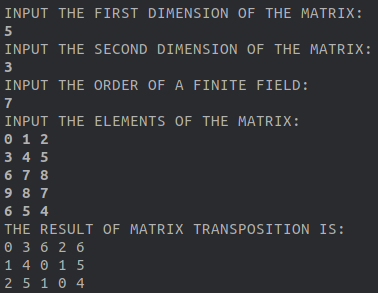
\includegraphics[scale=0.6]{matrix_field_transposition.png}
  \caption{Результат транспонирования матрицы в конечном поля порядка 7.}
\end{figure}

\par Результатом транспонирования матрицы $A$ размерности 5 $\times$ 3 является
матрица $A^{T}$ над конечным полем порядка 7 размерности 3 $\times$ 5. \\

\par \tbf{Оценка временной сложности алгоритма транспонирования матрицы в
  конечном поле.}
\par Оценим временную сложность алгоритма на примере матрицы $A$ размерности $N
\times M$ и порядка поля $ord$. После транспонирования матрицы $A$ и построения
матрицы $A^{T}$ над конечным полем порядка $ord$ число элементов в матрице $A^T$
будет соответствовать числу элементов в матрице $A$. Поскольку меняется только
размерность матрицы, а сами элементы лишь меняют своё расположение, то получаем
оценку временной сложности алгоритма: $T(get\_matrix\_field\_transposition) = O(N
\cdot M)$.

\newpage

\subsection{Алгоритм обращения матрицы над конечным полем}
\par \tbf{Описание алгоритма обращения матрицы над конечным полем.} \\
\tbf{Вход:} квадратная матрица $A$ размерности $N \times N$ над множеством
натуральных чисел и натуральное число -- порядок поля $ord$. \\
\tbf{Выход:} квадратная матрица $A^{-1}$ размерности $N \times N$ над конечным
полем порядка $ord$ -- обратная к $A$ матрица или сообщение о том, что матрица
$A$ является вырожденной. \\
\tbf{Метод:} сначала вычисляется определитель $\det A$ исходной матрицы $A$.
Если он кратен порядку поля, то матрица $A$ является вырожденной, и выполнение
программы прекращается. Иначе формируется сопряжённая к $A$ матрица $A^{*}$ --
матрица алгебраических дополнений. По расширенному алгоритму Евклида для $\det
A$ в поле заданного порядка ищется обратный элемент, который умножается на
$A^{*}$. Если какой-то элемент в получившейся матрице отрицательный, то
обновляем его значение по следующей формуле: $matInverse[i][j] = (matInverse \;
\% \; fieldOrder) + fieldOrder$.

\par \tbf{Псевдокод алгоритма обращения матрицы над конечным полем.}
\begin{lstlisting}[caption=Псевдокод алгоритма., mathescape]
matrix_field_inversion(<N$\times$M matrix> mat, unsigned int fieldOrder)
{
  det = (compute_det(mat) % fieldOrder) + fieldOrder;
  if (det % fieldOrder == 0):
    return;
  detFieldInverse = get_field_inverse(det, fieldOrder);
  <N$\times$N matrix> conjugateMatrix = get_conjugate_matrix(mat);
  return (remove_negatives(detFieldInverse * conjugateMatrix, 
                           fieldOrder));
}
\end{lstlisting}

\par В программной реализации алгоритма в качестве вспомогательных используются
следующие функции: $getMinor$, извлекающая необходимый минор при вычислении
определителя, $gcdExtended$, реализующая расширенный алгоритм Евклида нахождения обратного к
вычисленному определителю элемента в конечном поле заданного порядка,
$getMinorExtended$, извлекающая необходимый минор при построении матрицы
алгебраических дополнений 

\newpage

\par \tbf{Код программы обращения матрицы над конечным полем.}
\begin{lstlisting}[caption=Код программы., mathescape]
vector<vector<int>> getMinor (int columnIdx,
                              vector<vector<int>> matrix)
{
  int i, j;
  vector<vector<int>> minor;
  for (i = 1; i < matrix.size(); ++i)
    {
      vector<int> row;
      for (j = 0; j < matrix.size(); ++j)
        if (j != columnIdx)
          row.push_back (matrix[i][j]);
      minor.push_back (row);
    }
  return (minor);
}

int computeDet (vector<vector<int>> matrix)
{
  if (matrix.size() == 1)
    return (matrix[0][0]);
  int det = 0, multiplier = 1, i;
  for (i = 0; i < matrix.size(); ++i)
    {
      int elt = matrix[0][i];
      if (elt != 0)
        det += multiplier * elt * 
                            computeDet (getMinor (i, matrix));
      multiplier *= -1;
    }
  return (det);
}

void gcdExtended (int a, int b, int& x, int& y)
{
  if (a == 0) { x = 0; y = 1; return; }
  int x_1, y_1;
  gcdExtended (b % a, a, x_1, y_1);
  x = y_1 - (b / a) * x_1;
  y = x_1;

  return;
}

vector<vector<int>> getMinorExtended (vector<vector<int>> matrix,
                                      int rowIdx, int colIdx)
{
  int i, j, matrixSize = matrix.size ();
  vector<vector<int>> minor;

  for (i = 0; i < matrixSize; ++i)
    {
      if (i == rowIdx) continue;
      vector<int> row;
      for (j = 0; j < matrixSize; ++j)
        {
          if (j == colIdx) continue;
          row.push_back (matrix[i][j]);
        }
      minor.push_back (row);
    }
  return (minor);
}

vector<vector<int>> getConjugateMatrix (
  vector<vector<int>> matrix)
{
  int i, j;
  short sign = 1;
  bool evenDimensionFlag = (matrix.size () % 2 == 0);
  vector<vector<int>> conjugateMatrix (
    matrixDimension, vector<int> (matrixDimension, 0));

  for (i = 0; i < matrixDimension; ++i)
    {
      for (j = 0; j < matrixDimension; ++j)
        {
          conjugateMatrix[i][j] = 
            sign * computeDet (getMinorExtended (matrix, i, j));
          sign *= -1;
        }
      sign *= (evenDimensionFlag ? -1 : 1);
    }
  return (transposeMatrixMachinerie (conjugateMatrix));
}

void reduceMatrix (
  vector<vector<int>>& matrix, int fieldOrder, int detInverse)
{
  int i, j;

  for (i = 0; i < matrix.size (); ++i)
    for (j = 0; j < matrix.size (); ++j)
      {
        matrix[i][j] *= detInverse;
        matrix[i][j] %= fieldOrder;
        if (matrix[i][j] < 0)
          matrix[i][j] += fieldOrder;
      }
}

void invertMatrix ()
{
  unsigned int fieldOrder;
  int det, detInverse = 0, dummyVariable = 0;
  vector<vector<int>> inputMatrix, conjugateMatrix;

  cout << "INPUT THE DIMENSION OF YOUR MATRIX:\n";
  cin >> matrixDimension;
  cout << "INPUT THE FIELD ORDER:\n";
  cin >> fieldOrder;
  cout << "INPUT YOUR MATRIX:\n";
  getMatrix (inputMatrix);

  det = computeDet (inputMatrix);
  if (det % fieldOrder == 0)
    {
      cout << "MATRIX HAS ZERO DETERMINANT.
        INVERSE MATRIX CANNOT BE FOUND.\n";
      return;
    }
  det = (det % fieldOrder) + fieldOrder;
  gcdExtended (det, fieldOrder, detInverse, dummyVariable);
  conjugateMatrix = getConjugateMatrix (inputMatrix);
  reduceMatrix (conjugateMatrix, fieldOrder, detInverse);
  cout << "INVERSE MATRIX IS:\n";
  displayMatrix (conjugateMatrix);
}
\end{lstlisting}

\par \tbf{Результат тестирования программы обращения матрицы над конечным
  полем.}
\par Рассмотрим невырожденную квадратную матрицу $A$ размерности $N \times N$ в
конечном поле порядка 37. Найдём обратную к $A$ матрицу.

\begin{figure}[h!]
  \center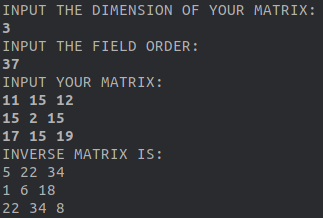
\includegraphics[scale=0.6]{matrix_field_inverse.png}
  \caption{Результат обращения матрицы в конечном поле порядка 37.}
\end{figure}

\par Проверим, что полученная матрица действительно является обратной к $A$. При
умножении исходной матрицы и полученной должна получиться единичная матрица.

\begin{figure}[h!]
  \center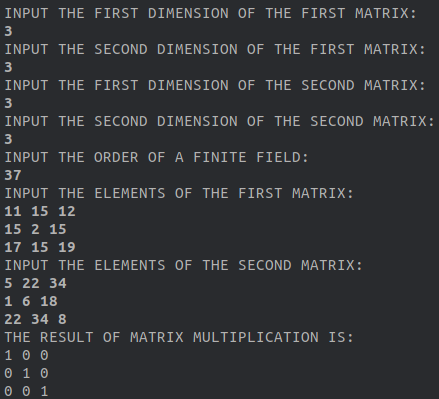
\includegraphics[scale=0.5]{matrix_field_check.png}
  \caption{Проверка корректности нахождения обратной матрицы.}
\end{figure}

\par \tbf{Оценка временной сложности алгоритма обращения матрицы в конечном
  поле.}

\par Будем рассматривать невырожденную квадратную матрицу $A$ размерности $N \times
N$ с порядком поля $ord$.
\par Будем оценивать сложность алгоритма в соответствии с операциями,
упомянутыми в псевдокоде.
\par Первая операция -- нахождение определителя матрицы $A$. Для нахождения
определителя матрицы порядка $N \times N$ методом Лапласа (разложением по строке
или столбцу) необходимо вычислить значения $N$ миноров $N - 1$ порядка.
Вычисление будет продолжаться, пока миноры не станут 1-го порядка
(одноэлементные матрицы). Следовательно, временная сложность операции вычисления
определителя матрицы порядка $N \times N$ составляет: $T(compute\_det, N) =
O(N!)$.

\par Вторая операция -- нахождение обратного к определителю элемента в конечном
поле заданного порядка. Обратный элемент ищется по расширенному алгоритму
Евклида. Временная сложность выполнения этой операции составляет:
$T(gcdExtended) = O(\log b)$, где $b$ -- наименьшее из двух входящих значений
(оценка сложности получена в книге: Knuth, Donald. The Art of Computer Programming. Addison-Wesley. Volume 2,
Chapter 4).

\par Третья операция -- построение сопряжённой матрицы. Аналогично вычислению
определителя матрицы, только теперь дополнительный минор должен быть вычислен
для каждого элемента исходной матрицы. Таким образом, временная сложность
операции построения сопряжённой матрицы составляет: $T(get\_conjugate\_matrix) =
O((N!)^2)$, где $N$ -- размерность исходной квадратной матрицы.

\par Заключительная операция -- проход по получившейся матрице с целью
замены отрицательных элементов на элементы поля заданного порядка. Временная
сложность: $O(N^2)$.

\par Таким образом, сложность алгоритма обращения невырожденной квадратной
матрицы размерности $N \times N$ в конечном поле:
$T(get\_inverse\_field\_matrix) = O((N!)^2)$.

\newpage

\conclusion

\par В ходе лабораторной работы мною были изучены основные понятия универсальной
алгебры и операции над бинарными отношениями. В качестве практического задания
мною были описаны и реализованы алгоритмы проверки основных свойств операций по
их таблице Кэли, алгоритмы построения объединения, пересечения, дополнения,
композиции и обращения бинарных отношений, а также алгоритмы сложения,
умножения, транспонирования и обращения матриц в полях конечного порядка. Для
этих алгоритмов были представлены псевдокоды, осуществлена их программная
реализация, а также проведена оценка временной сложности.

\end{document}